%===================================== CHAP 2 =================================

\chapter{Literature Review}
This project's objective is to look at how the construction industry, or precisely how LVB, make use of Lean Construction and digital tools to aid project management. The CI's lust for digitalization is ever-present, and often projects consist of entire departments responsible for digitalization. This chapter is using ICT as a successful case of utilization of digitalization in the context of agile project management. 

First, the chapter takes a historical look at ICT and CI, and which factors made both utilize agile project management in the first place – what were the symptoms needed to be fixed? This comparison gives a surprisingly similar line of arguments, where productivity, complexity, failing to meet budgets, and requirements change during project implementation are some — additionally, similarities between the project process address comparison. 

Secondly, discussing organizational cooperation and interaction, where one looks at software as a tool aiding organizational interaction. Furthermore, the chapter gives a brief overview of a traditional CI project, as well as a short overview of different agile project management methods as a context for the project.

\section{A Brief History of Software Engineering}
Software engineering is considered one of the newer disciplines of engineering. From 1842, when Ada Lovelace first described the advantages of the Analytical Engine, up to the 1968 NATO Garmisch conference, computer science was not considered an engineering field at all. Back then, engineers found writing code a handcraft, done by the specialists, that could be applied in several disciplines of engineering. 

By the 1950s, military initiatives had seen the need for some structure or process that could aid large-scale development. Because there was no standard procedures the industry suffered significant productivity issues. The process used back then is now known as the code-and-fix method. Problems using this method was: (a) products not hitting the needs of the user, (b) code that was barely readable, and (c) not testable. Also, producing software with a team was shown difficult because of a lack of documentation and inexperienced team members. 

In 1956 H.D. Bennington wrote a paper: "Production of Large scale Programs." Bennington proposes, among other things, an operational plan. The operational plan included nine phases to prepare a large system program, seen in figure \ref{fig:bennington}. The plan is considered the precursor of the waterfall model, introduced by W.W. Royce, with the "Managing the Development of Large Software Systems"-paper, from 1970. What Royce is describing is a way of managing large-scale software development within both cost and time. The Waterfall has since become the dominant software development method used in the industry. The problems both Bennington and Royce saw was the need for process management. The reason for the need for process management was that programs did not meet cost- and time schedule, as well as requirements set. The industry suffered major productivity issues. The resulting product did not meet the expectation of the user, and the requirements needed to be modified, or the development process had to return to the origin. The issues had the source of poorly designed and documented requirements. The need for documentation and requirement specification features that come in to play in more complex software developments, because one could not see the bigger picture when the complexity of the program increased to a certain level.

\begin{figure}
    \centering
    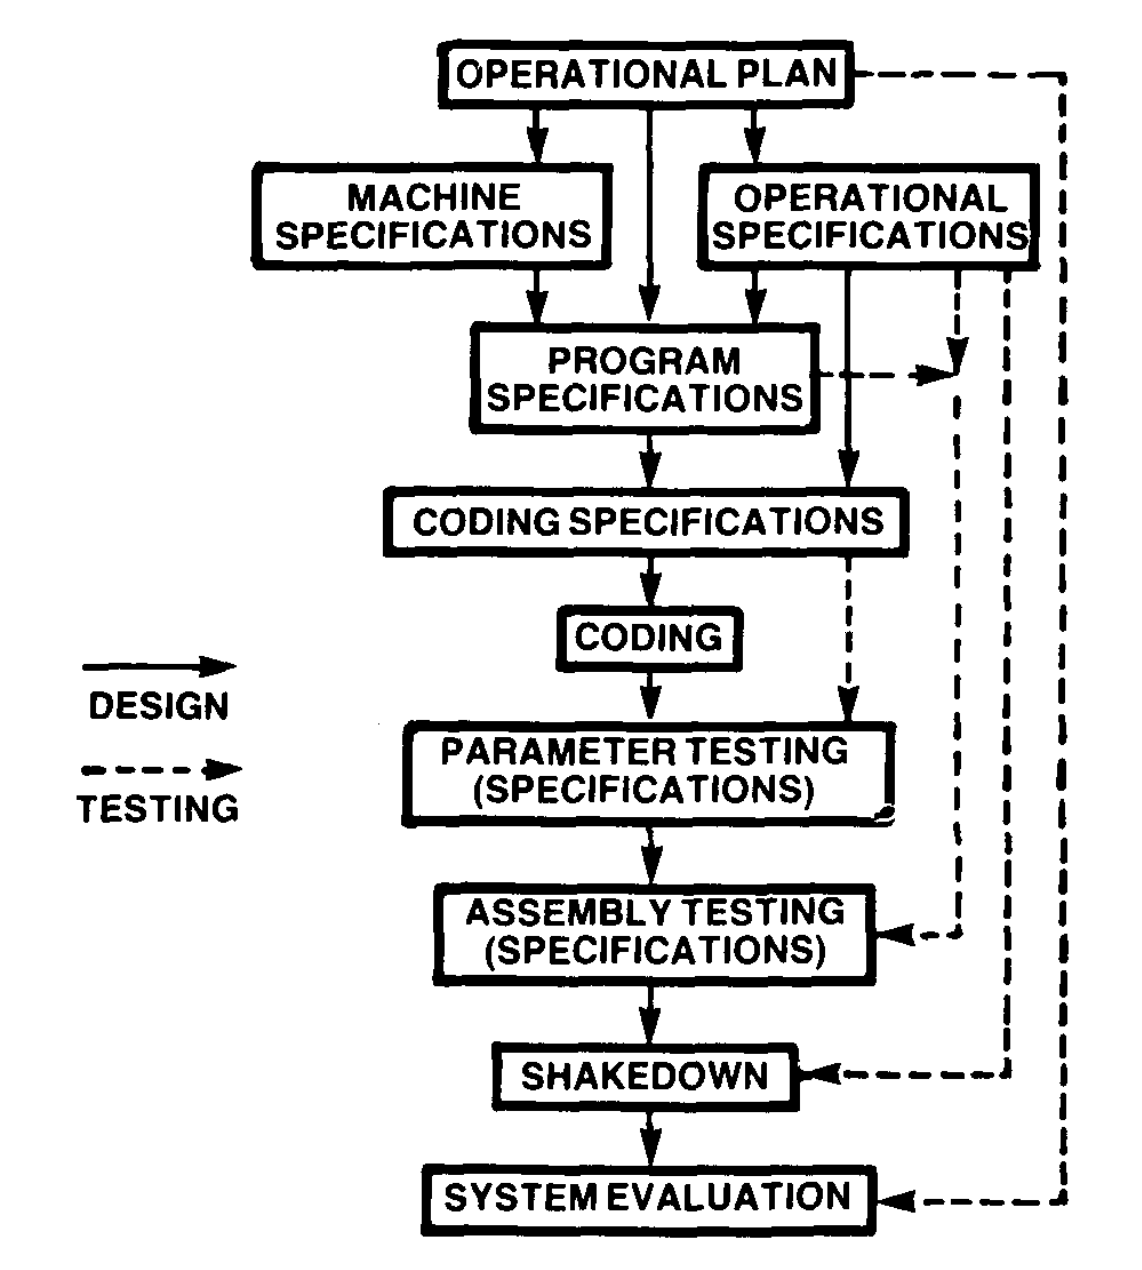
\includegraphics[width=0.55\textwidth]{fig/bennington-production-of-large-scale-programs.png}
    \caption{Production of a large-program system as presented of Bennington in 1956.}
    \label{fig:bennington}
\end{figure}

Further, one wanted to make sure that the code written was performing as intended, which introduced the need for testing. The waterfall model, presented by Royce, seen in figure \ref{fig:royce}, has some modifications to Bennington's Program production, but one can identify notable similarities between the two. A feature for them both is that, to some extent, they proclaim the use of an iterative design process, which has shown to be forgotten in recent years, using the waterfall model. Royce shows the prototype in a illustration, seen in figure \ref{fig:royce-prototype}, while in Bennington's paper the iteration is not mentioned, but he does indicate the use of iterations in the later applied foreword.

\begin{figure}
    \centering
    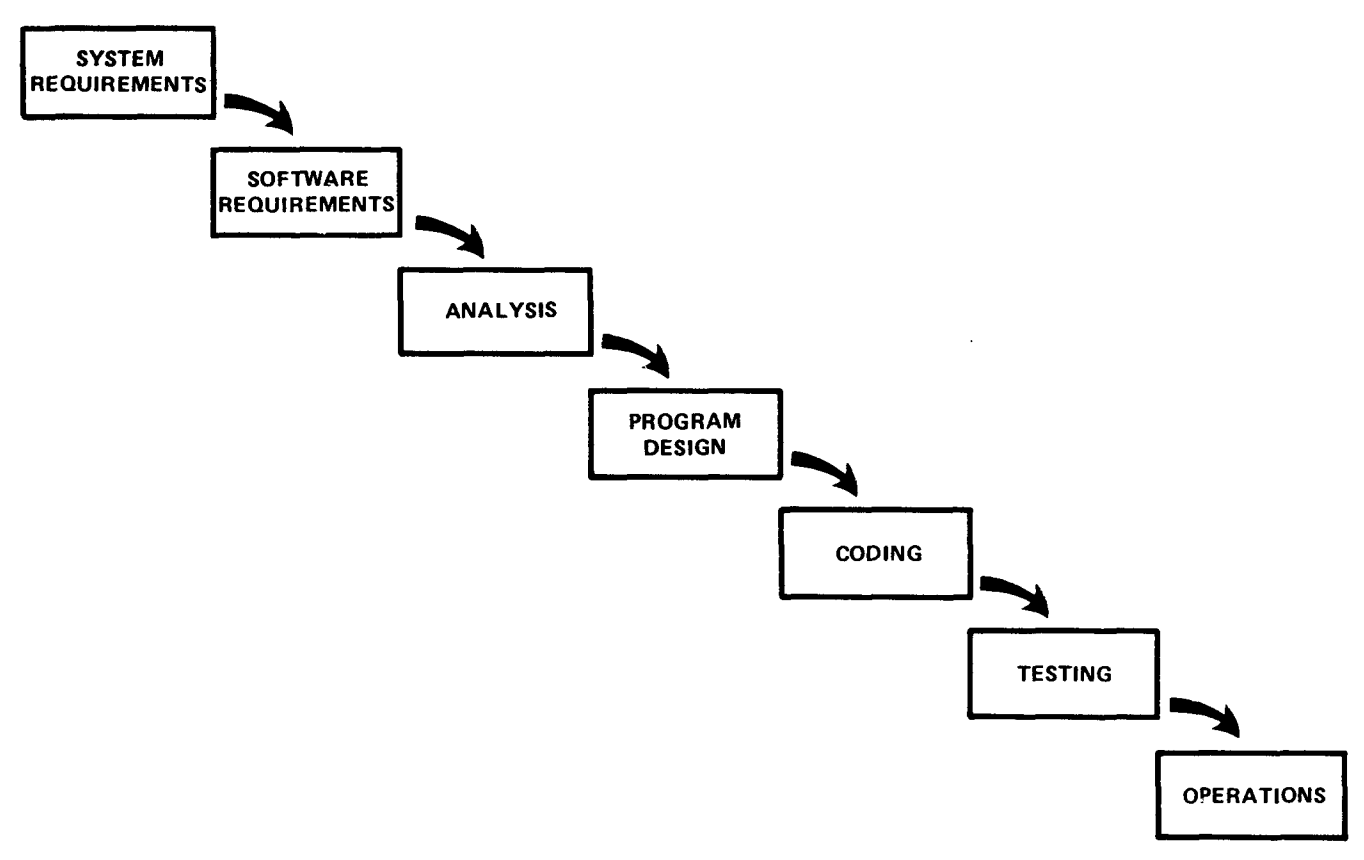
\includegraphics[width=0.8\textwidth]{fig/royce-waterfall.png}
    \caption{Waterfall method as proposed by Royce in 1970. Visualizing implementation steps to develop a large computer program for delivery to a customer.}
    \label{fig:royce}
\end{figure}

\begin{figure}
    \centering
    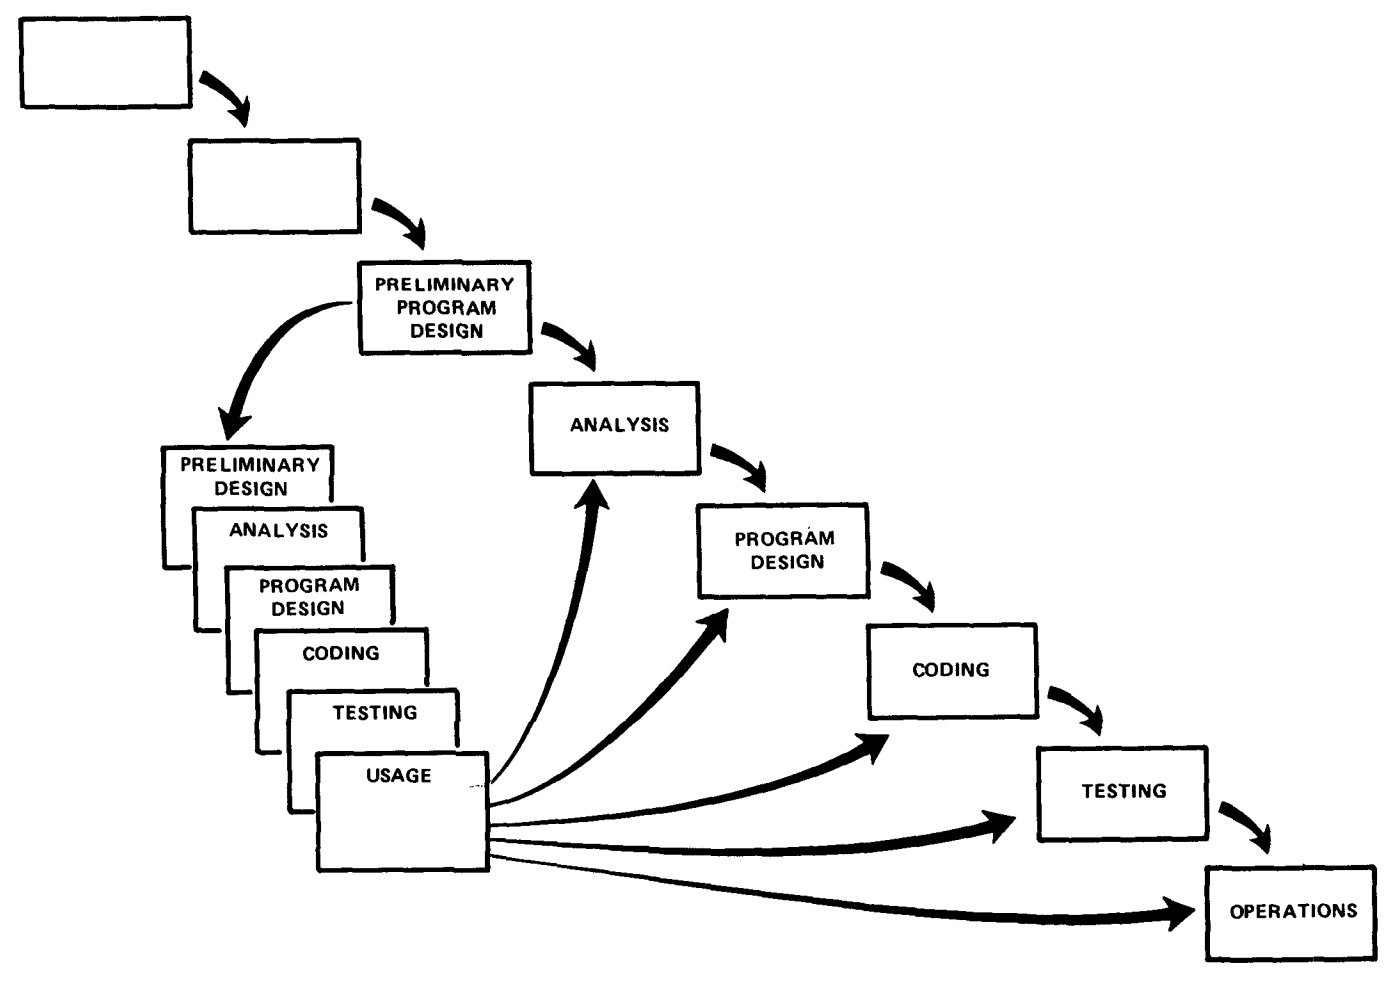
\includegraphics[width=0.8\textwidth]{fig/royce-waterfall-prototype.png}
    \caption{Waterfall method as proposed by Royce in 1970, including an iterative process using prototype. Attempting to do the job twice - the first result provides an early simulation of the final product.}
    \label{fig:royce-prototype}
\end{figure}

In 1987 Barry W. Bohem wrote a paper comparing three papers from the past, with how the software industry treats process management of the time. The papers compared includes both Royce's and Bennington's paper. Bohem starts the paper with a quote from Gorge Santayana, "Those who cannot remember the past are condemned to repeat it." Even after Royce, the industry still struggled with requirements, documentation, staffing, and testing. Following the process, but forgetting the details resulting in some of the same problems previously recorded, thus the Santayana quote. An interesting detail is Bohem's discovery of the lack of prototyping and iteration, in the interpretation and use of the waterfall model: "Thou shalt not write one line of code until every detailed design specification is completed;" though both Royce and Bennington promote prototyping in the design phase. 

The industry, entering the 90s and the 21 century, had a set of structures, processes, and models. Furthermore, it had become a known and highly valued field of engineering. Still, the discussion of productivity- and efficiency was present. Large software developments failed to deliver at the time and cost initially planned, sometimes failing to deliver at all.  Some of the repeating problems were: (1) the initial requirements often changed during the development process: forcing the development going back to the origin, costing both time and money; (2) the need of project management during a stage of the process: making sure developers working in parallel being exploited at an accepted level, and knowing what to implement at all times. The process models, such as Waterfall, structure the order of stages, and when to proceed to the next stage, while process methods are more concerned about guidance through each phase. Thus the need for software management methods was present and the introduction of Agile Development as a means to overcome, among others, the two problems mentioned. 

One can argue that productivity is an ever fighting battle, but after the introduction of agile development, productivity is shown to have a definite increase in Norwegian ICT-industry. Looking at figure \ref{fig:ICT_BA_1972}, comparing ICT and CI, the difference is substantial. Yes, the productivity of CI is not good, but a productivity gain of 478,9\% from 1972 until 2017 is to be considered satisfactory. One can see a big leap from the middle of the 90s. Using Labor Productivity measuring how a industry is discussed later in this chapter.

\begin{figure}
    \centering
    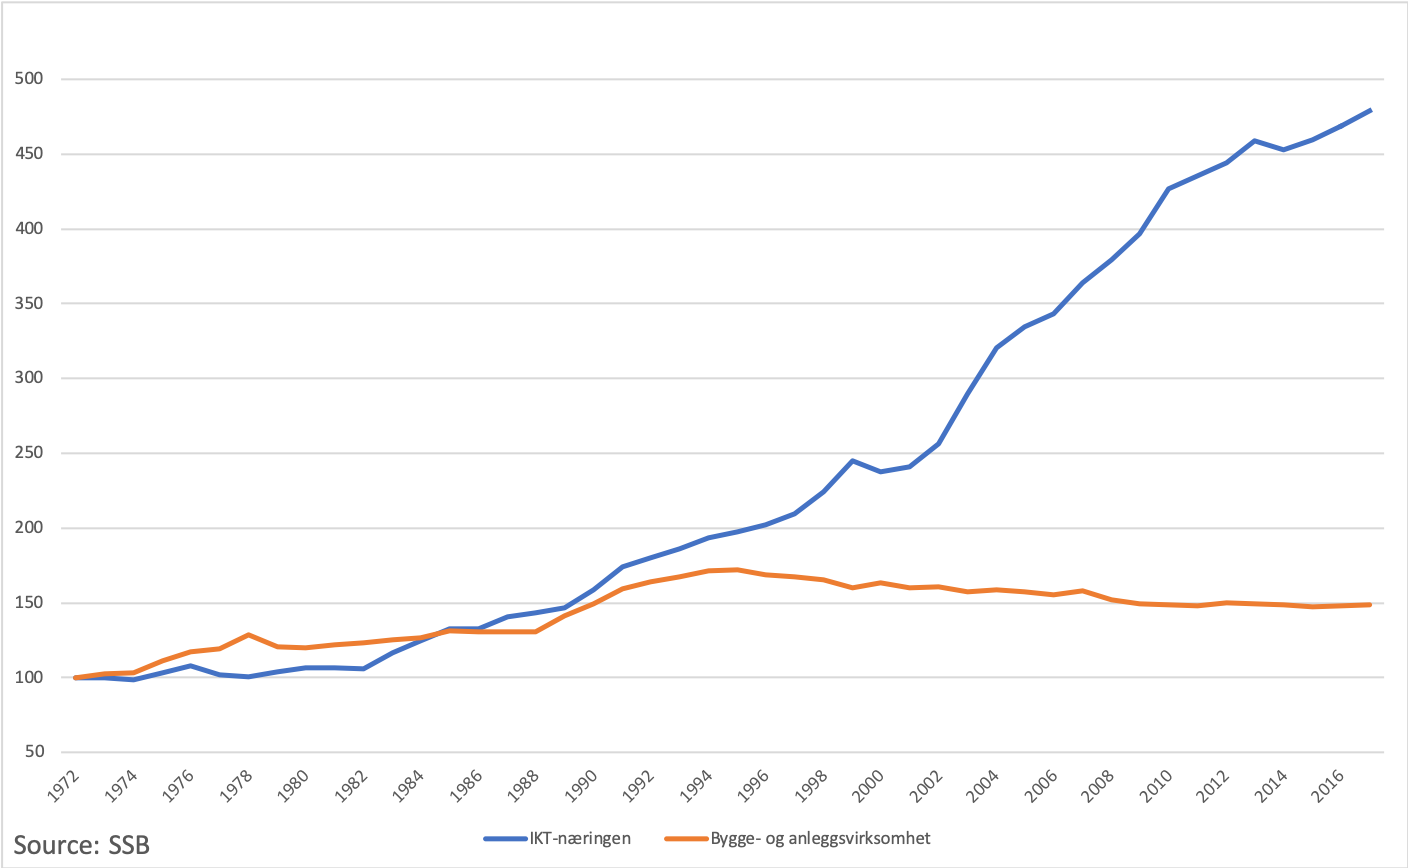
\includegraphics[width=\textwidth]{fig/ICT_BA_1972.png}
    \caption{Labor productivity; ICT and CI compared from 1972 up to 2017.}
    \label{fig:ICT_BA_1972}
\end{figure}

\section{Construction Engineering}
Construction Engineering has been a significant field of engineering throughout history. Originates from the construction of the pyramids. Continuing with Da Vinci, and some of the most skilled people, in the middle ages, forming some of the most known structures of today. In the raging of wars and through the industrial revolution, one could witness the rapid development of both civil and military engineering; as a result, one could now construct both faster and better than ever before.

Over the last century, the requirements of constructions have become more and more complex. The buildings are getting higher, the tunnels are getting longer, and the roads are getting wider. The size of things is not equal to the complexity of the construction. Adding automated systems, multipurpose functionality, and multiple communication platforms, the complexity is ever so present. Take for example a university building, which is no longer simply a place where one can lecture and read. A university building now requires to host highly sophisticated labs for various purposes, as well as several other rooms for different kinds of purposes, and some also multipurpose. Besides, that is just the requirement of the rooms; one needs to consider all the systems added in regards to, among others, ventilation, electricity, sewage treatment, internet, and telecommunication. All these systems- and room requirements, as well as other requirements, makes the construction of the modern building way more complicated than it used to be. 

Even though the complexity of the construction is increasing, the process management has, for the most part, been the same — resulting in an unfortunate progress of productivity in CI. 

\subsection{Construction Industry Project as Context for the Project}
The process of constructing, in Norway, follows a pattern described by The Norwegian standard agreements (SSA). The construction process divides into five steps: (1) the early phase: where deciding both the vision of the project and process of project conduction; (2) the procuring of architect or adviser: starting by publishing the project and at the end awarding the best actor with a contract; (3) the design phase: where one produces different levels of  design; (4) the procuring of entrepreneur(s): includes deciding on contracts, and choosing the correct contractors for the job; and (5) realization: where conducting the substantive implementation. 

The third phase, designing, is typically conducted in three levels of granularity. First, the architect is sketching the over-all concept of the construction and delivering the concept as a set of drawings, models, and specifications. Furthermore, the concept is to realize the intention and vision of the project. Second, often called the pre-project, a team often consisting of architects, project managers, and engineers, is to define the project. The definition results in a set of user- and technical requirements, as well as further developing the functional and physical structure of the project. It is here one sets the budget and goals of the project. The pre-project is ending by handing the result and a proposal of decision for political treatment. The political treatment is known to be time-consuming, often spanning a one-to-two year period. Given the political decision, the requirements and budget set, limits and sets the basis for the rest of the project, as well as the goals used to measure. Third and finally, the detailed design is happening. The result of the detail design is the sketches used in the procurement of contractors — plus, an outline of the awarding strategy used in the next phase. Because of the time-consuming political decision, a new team is often responsible for the detailed design. Documentation of the pre-project is therefore vital. When going into the realization, it is the detail-design-team that is responsible for the project to keep the budget and achieving the goals set by the political decision, which can seem unfair if the pre-project requirements are not manageable.

A typical case is a change of requirements, required by a stakeholder, either during detailed planning or the production-phase. A change often leads to budget-breach, or if not feasible, dissatisfied stakeholders. 

\subsection{Productivity}
The Norwegian CI is, as mentioned, accused of having a decline in Labor Productivity (LP). An Industry that is one of the most significant industries in On-Land Norway, with 466 billion Norwegian Kroner accumulated in 2017. A common fact shared among the industry stating that CI is facing an LP decline of 10\%, since the year of 2000. Often these numbers are justified by a complex and ever-changing industry and considered not representative of the industry of today. Sure the numbers are correct, but do these numbers show us the big picture?

In this section, the question of declined LP in Norwegian CI will be discussed, and if LP is in fact \textit{not} declining.

Labor productivity(LP) is a description of the value created relative to the resources used, as seen in equation \ref{eq:labor_prod}. Practically speaking, a company or business achieving a high degree of LP, work less, and achieve more. 

\begin{eqnarray}\label{eq:labor_prod}
Labor Productivity = \frac{\textit{Labor dividends in quantity or value}}{\textit{Labor effort in hours or count of employees}} 
\end{eqnarray}

Having increased productivity, make sure that a company gets the right turn on investment, rather than barely be able to endure. There are lots of different factors that come in to play why some industries have a positive LP-rate, and some have a negative LP-rate, but how can this decline be, when the Industry see turnover growth?

\begin{figure}
    \centering
    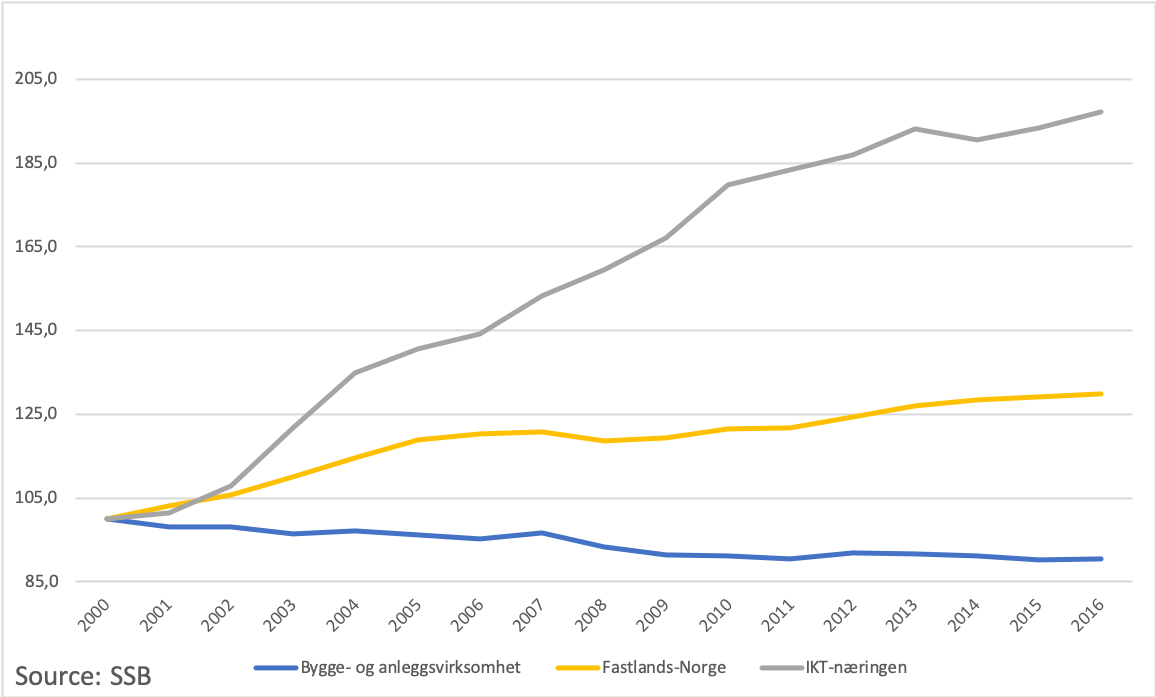
\includegraphics[width=0.9\textwidth]{fig/ba_on-land_ICT.png}
    \caption{Labor productivity in the constructing industry, compared to average on-land industries in Norway, from 2000 to 2016.}
    \label{fig:productivity-comparing}
\end{figure}

By Statistics Norway (SSB) the constructing Industry (CI) suffer a substantial decline of 10\%, since the year of 2000. This trend is also present in both Sweden and Finland. Comparing these numbers, seen in figure \ref{fig:productivity-comparing} with the same statistics in LP in all on-land private sector businesses, where there has been an overall increase, by 30\%, one can arguably state that the decline is a fact. What do these statistics represent? SSB' definition of CI used in this calculation is labor that is directly involved in the on-site constructing, which is not representative of what is considered CI of 2019. Much of the work done on today's building site is prefabricated, and to get construction completed, one has to cooperate with a lot of businesses and industries. SSB explains that the reason for the small definition of CI is because of an EU-standard; hence, the comparison of the northern countries. If we consider the entire supply chain, there is a minor, in fact, increase in productivity of about 2\% from 2000 to 2016, as seen in figure \ref{fig:LP_supply_chain}.

\begin{figure}
    \centering
    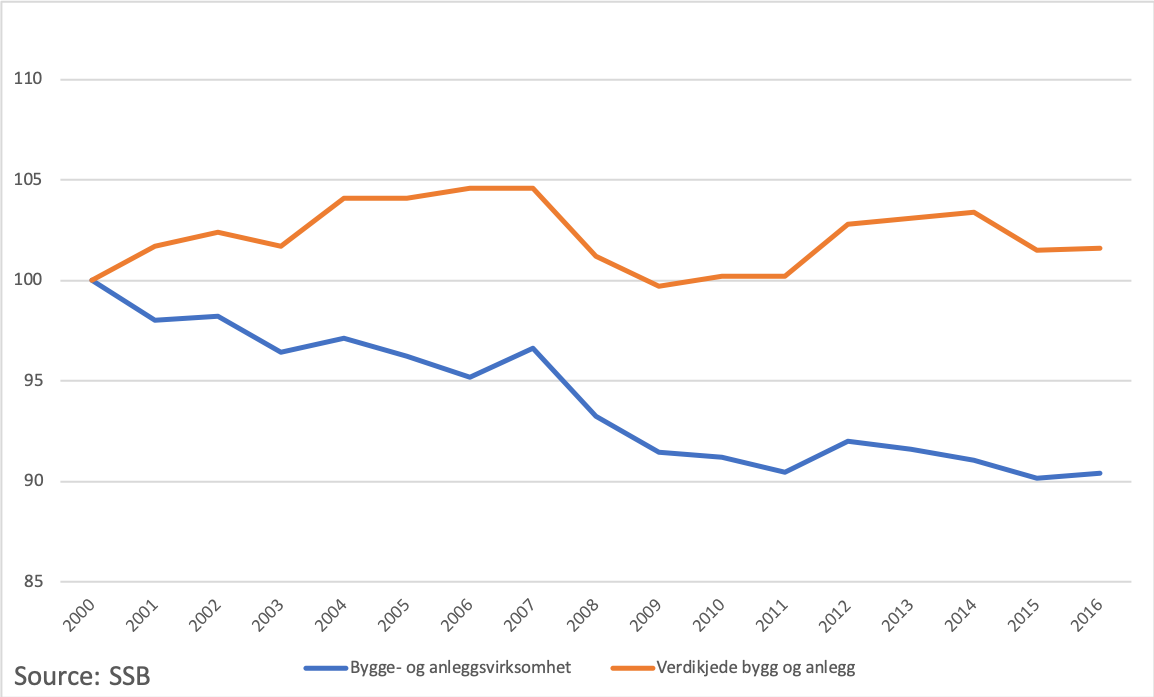
\includegraphics[width=0.9\textwidth]{fig/ba_value_chain.png}
    \caption{Labor productivity in the constructing industry supply chain, from 2000 to 2016.}
    \label{fig:LP_supply_chain}
\end{figure}

An issue paper posted by Sintef in 2013 raises the discussion about this topic. The issue paper states three central observations: (1) The numbers does not tell the whole story about productivity, (2) the numbers can’t be used in scientific research and (3) the numbers can not be used in comparing businesses, projects or corporations, because each project is so vastly different from one another. 

Looking at observation two, stating that the numbers are not to be used, measuring increased productivity in CI overall. We need, therefore, to look at a process, a specific project, or a corporation to conduct a sufficient scientific analysis. This holds for a case study, where one looks at an individual project, analyzing the internal processes and project management to identify the measurements taken to boost internal productivity. Moreover, complexity makes for no comparison between different projects, because when creating a complicated construction, sometimes new invention needs to happen, and this is not something to be compared. In the same way, comparing productivity in different software development projects is not relevant. If one is to construct the same house, or the same piece of software, time after time, then a comparison is very legit. Then again, in this case, the ingenuity is discussable.

Stating that CI has declining Labor Productivity is therefore not unilaterally correct - still, if we consider the total value chain, the result is considered poor. The industry is taking action to get labor productivity closer to the average rate. The focus is to make each project as efficient and productive as possible, but that is always the case. Simply because of the marginal cost gained.

Thus yields for a bottom-up approach: Starting with a process in a project and perfecting it, continuing with each process will eventually lead to a resulting better efficiency and productivity in the entire project.  Which, if done in the entire constructing industry, will lead to increased LP overall. Therefore, the industry needs to overcome the challenges, (starting with a breach of planned timeline and budget, with symptoms such as requirements change during design, increased complexity, and struggling to complete the products) mentioned earlier, were digitalization, Agile, and Lean is promising and populare solutions to the problem. 

\subsubsection{Measuring productivity on project-, process- and process level}
Practicing the bottom-up approach and implementing Lean Constructing in the design- and implementation phase, increasing productivity, and overcome difficulties (such as requirements change during design, increased complexity, and breach of planned timeline and budget) within the particular project phases. Lean is an excellent method but offers no mechanism measuring the achieved improvements. Using KPI's measuring could be a solution. Skappel \cite{skappel} suggests in her master thesis, ten KPIs ensuring continuous flow improvement in Lean design process: 
\begin{enumerate}
    \item Number of work packages (deliveries) completed and delivered within a takt time
    \item  Number of decisions made on the wrong basis
    \item  Number of revisions after products in a common BIM are frozen
    \item  Number of unresolved questions in the dialog matrix
    \item  Intensity Curve - Number of questions asked in the dialog matrix and how fast these are
    resolved
    \item  Number of approved functional descriptions prepared at the right time
    \item  Number of correct functional descriptions revealed during table testing
    \item  Number of systems with developed test procedures before sending contract to contractors
    \item  Number of change requests due to errors and misunderstandings
    \item  Percentage of project material delivered to the contractors at the right time
\end{enumerate}
These KPIs are yet to be tested, but still promising ensuring LP in the first phase of a traditional CI-project evolve in the appropriate direction. 

In addition, by recommendation of the issue paper a project, started in 2015, establishing a state-of-the-art performance measurement tool. In 2017 the resulting Nordic 10-10 \cite{nordic-10-10} program was finished. Nordic 10-10 is a version of the CII 10-10 program\cite{CII-10-10}, designed and translated for the Nordic countries. The CII 10-10 program is a survey-based measurement tool based on the concept of anonymously surveying members of a project, regarding their project's performance, team dynamic, and organizational relationship. The surveying is done at the end of each of the five faces of the constructing project. Opposite to a standard approach, where such analysis is done only one time; at the end of the project. Using Nordic 10-10 results in more agile project management, where changes are implemented throughout the project. In some projects, they even do the analysis even more often, allowing the project manager to make changes also within each phase of the project. 

As mentioned, the use of process management and method management has helped ICT and software development. If not directly increasing LP, although structuring projects, increasing interactions, and overcome the challenges in SD and curing the symptoms seen both in ICT-industry and the CI.  

Since the introduction of SCRUM \cite{scrum}, in 1995, the use of it, and other SDM, has been wastly spread throughout the majority of software development projects in the world, and Norway as well. It is, therefore, fascinating looking at the figure \ref{fig:ICT_BA_1972}. Comparing LP in ICT and CI from 1972, up to the beginning of the '90s. Sky-rocketing after dot com, at the beginning of this century, while CI has a slight declining graph after breaking the millennia. Knowing the Agile manifesto was published in 2001 makes for a promising correlation. Though, one can not use LP as a single source of indication, nor stating that SDM is the single reason for the progress; this result yields for implementing agile project management in other industries. The next section will, accordingly, introduce different agile project methods.

\begin{figure}
    \centering
    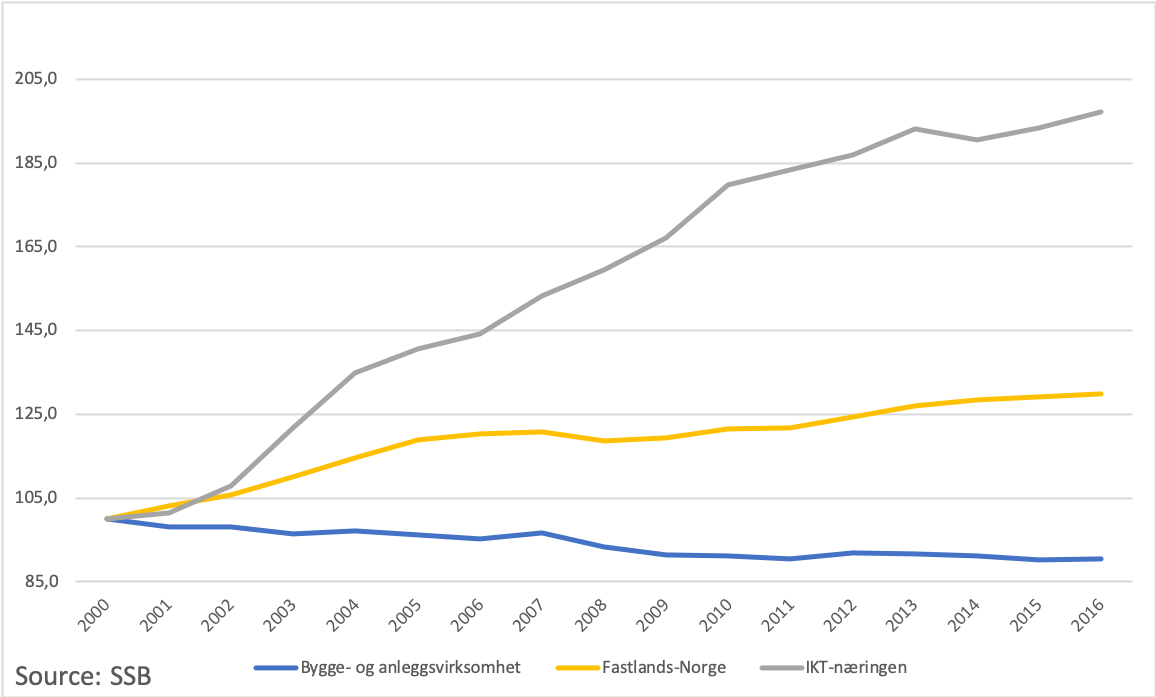
\includegraphics[width=\textwidth]{fig/ba_on-land_ICT.png}
    \caption{Labor productivity in ICT, compared to constructing industry and average on-land businesses in Norway, from 2000 to 2016.}
    \label{fig:LP_ICT_VS}
\end{figure}

\section{Project management methods}
\subsection{Agile Constructing}
\subsection{Agile Software Development}
Agile software development is a mindset and method, often conducted in iterations of a team of 5-12 people, to increase productivity and rapidly deliver value in the form of usable software. Often the Manifesto for Agile Development is used as a definition of agile. Several methods implement this manifesto. Some known methods are; Extreme Programming (XP), SCRUM, or Kamban. Large scale corporations may implement a uniquely customized method, or several of these methods, within the company. To state that one company is agile is therefore considered imprecise, one because of the number of team members, and second not everything the company conduct is done in an agile matter.
\subsubsection{SCRUM}
\subsubsection{Kanban}
\subsubsection{Lean}
\subsubsection{Agile software development in large scale corporations}

\section{Interaction}
The work of constructing a highly complex and costly structure is, as we have understood, difficult. There is no straightforward way of doing it, and the focus on project management is an essential part of it. Though, in the end, the act of design and project management is primarily making people work together. Make people interact, coordinate, and synchronize for them to create something that could not happen, if not cooperating. The challenge of making people meet and work together on a common goal, not being self-centered, is something the industry finds difficult. It is seen both in CI, in ICT, and most other industries that have to coordinate different domains of competence. 

This section will discuss this challenge and examine what the ground principals of cooperation are and look at different measures done, exposing it. How may computers support cooperative work? Furthermore, how do contracts influence the interest of different actors to cooperate? First, a short introduction to cooperation.

Cooperation is the act of communicating and share knowledge in a way that makes different actors coordinate, interact, and synchronize. The act of talking starts with a desire, or at least a reason, for various individuals to talk. One must take for granted that the lust is there, but in some cases, contracts, politics, or even physical barriers hamper this to happen. Regarding physical boundaries, the internet and telecommunication have been a significant leap forward towards decreasing this challenge. Computer-supported cooperative work (CSCW) is how technology supports teams cooperate in a project. CSCW will be discussed later in this section. Furthermore, this section will give a brief insight into Norwegian CI- contracts and politics as a context for the project. 

Secondly, the act of talking among project actors and team members is, in most cases, sharing knowledge. One often divides knowledge into tacit- and explicit knowledge. Tacit knowledge is something that is known to actors, but not written down, or otherwise, for somebody else to learn and understand. Where, on the other hand, explicit knowledge can be assimilated simply by reading a manual, or a document. Systemizing could help digest explicit knowledge because sometimes the information is there, but how to find it could be the impediment. In modern times computers are more and more often taken in to use, systemizing knowledge. The introduction of computers could lead to new tacit knowledge, on how to use the systems.

%Boundary Spanners and Boundary Objects

\subsection{Contracts in the Construction Industry}
The Norwegian standard agreements (SSA) dictate public procurement in Norway.  Following these laws, Agency for Public Management and eGovernment (Difi) has standardized e-procurement and contracts in the ICT-industry, which secure all parties involved in a given procurement. In CI, on the other hand, each party announcing procurements creates tailor-made contracts based on the Norwegian Standard (NS), e.g., NS 8405, NS 8406, and others. 

SSA's e-procurement process consists of three phases: (1) planning, (2) tendering, and (3) purchasing. The process obtains a simple procurement process, for both buyers and sellers. Including the process, there are also several standard contracts available, ensuring visibility and simplicity for all parties. The use of these contracts is widespread in the ICT industry. There is even a contract specially design for agile software development projects. In CI, SSA defines a five-step process including; (1) early phase, (2) procuring architect or adviser, (3) engineering, (4) procuring entrepreneur, and (5) realization. 

Contracts limit the ability to use agile methods. Difi's Agile contract (SSA-S) makes for an agile software process, consequently only made for ICT. An SD for agile construction is jet to be designed. 

Contracts who are different from one vendor to another makes for a challenging space of deals, for the entrepreneurs. This strategy helps larger companies or the ones who specialize in contracts from only a few vendors. A contractor who wants to earn a new principal has to learn the new contract, which favors the contractor who previously knows the contract and how it plays out. 

\subsection{CSCW}

\subsection{Interactions }


\begin{itemize}
    \item Konkurranse rundt for å vinne kontraktene: Noen kan spillet
    \item Entreprisemodeller
    \item Contracts
    \item påskuddskostnader
    \item Budjetter
\end{itemize}


\cleardoublepage